\section{Preliminary Results}

In this section, we evaluate the performance of the state-of-the-art robust
SLAM method, the Max-Mixture algorithm, given dynamic landmark measurements.
Max-Mixture is a robust extension to classical graph SLAM using Gaussian
mixture in factor representation, that is, $ x_i = \sum_c \phi_c
\mathcal{N}(\mu_c, \Sigma_c)$ for component $c$ and weight $\phi_c$, with
obvervations being components, also similarly for $z_i$. Max-Mixture uses a max
function to approximate and efficiently evaluate the sum of Gaussians. It is
well-known for its capability of handling a large amount of incorrect loop
closures, but it is untested against moving landmarks, and this experiment can
be representative to other approaches in the robust SLAM literature. 

We apply different perturbations to a single landmark (landmark 249) in the
Victoria Park dataset, and compare the different effects of the perturbations
on the optimal estimate of the trajectory and the map of all landmarks obtained
by Max-Mixture graph SLAM. The Victoria Park dataset contains 2-D odometry and
landmark observations. As shown in figure \ref{fig:baseline} the left plot is
the control group without perturbation, and is accurate to the ground truth. A
single southward bias is applied to all observations of the
landmark in the middle plot, simulating sensory outliers. A temporally
increasing bias is applied to all observations of the landmark in the right
plot, simulating a southward moving landmark.

\begin{figure}[h]
\makebox[\textwidth][c]{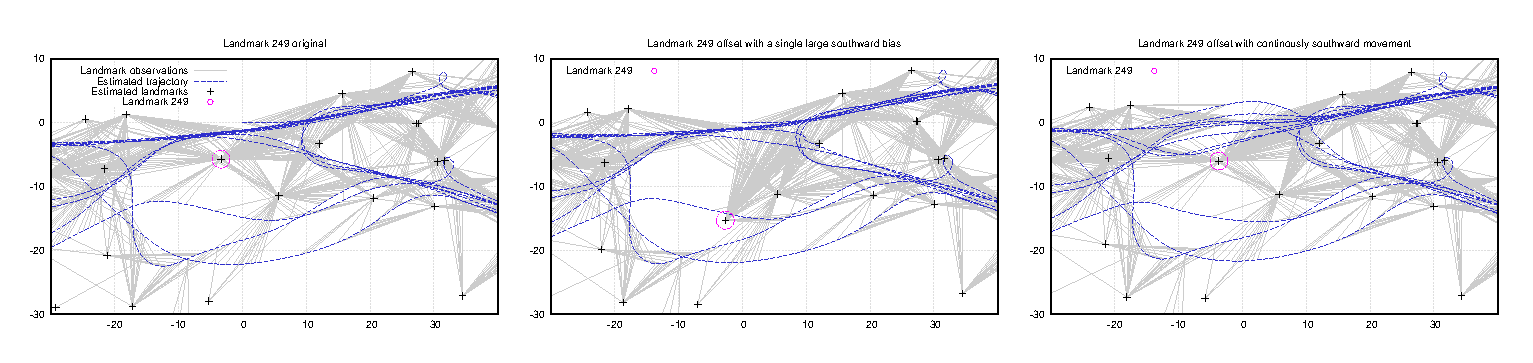
\includegraphics[width=\textwidth]{fig/baseline-mm}}
\caption{The optimal estimates of the trajectory and landmark positions
obtained by Max-Mixture graph SLAM.  Left: low convergence uncertainty. Middle:
high convergence uncertainty because of rejection of outlier observations
of landmark 249.  Right: low convergence uncertainty, no outlier
detected by Max-Mixture.}
\label{fig:baseline}
\end{figure}

As the middle plot shows, Max-Mixture is still capable of handling noise of
large bias or spurious loop closures introduced by simluated sensory fault. It
correctly rejects outlier landmark observations and recovers the position of
the perturbed landmark. However, it completely fails to reject any unlikely
landmark observations and largely distorts the resulting trajectory when given
moving landmark measurements. An explanation for this is that each clique of
landmarks with coherent motion forms a plausible reference frame for related
observations. Inference based on each independent reference frame will reach
plausible estimate of robot trjectory and the map, however robust SLAM methods
which assume stationary landmarks will average over a sum of different
reference frames and lead to wrong conclusions.

